%
% stereographisch.tex -- template for standalon tikz images
%
% (c) 2021 Prof Dr Andreas Müller, OST Ostschweizer Fachhochschule
%
\documentclass[tikz]{standalone}
\usepackage{amsmath}
\usepackage{times}
\usepackage{txfonts}
\usepackage{pgfplots}
\usepackage{csvsimple}
\usetikzlibrary{arrows,intersections,math}
\begin{document}
\definecolor{darkred}{rgb}{0.8,0,0}
\def\skala{1}
\begin{tikzpicture}[>=latex,thick,scale=\skala]
\pgfmathparse{atan(2.2)}
\xdef\w{\pgfmathresult}

\begin{scope}[xshift=3cm,yshift=5cm]
\node at (-0.8,0) {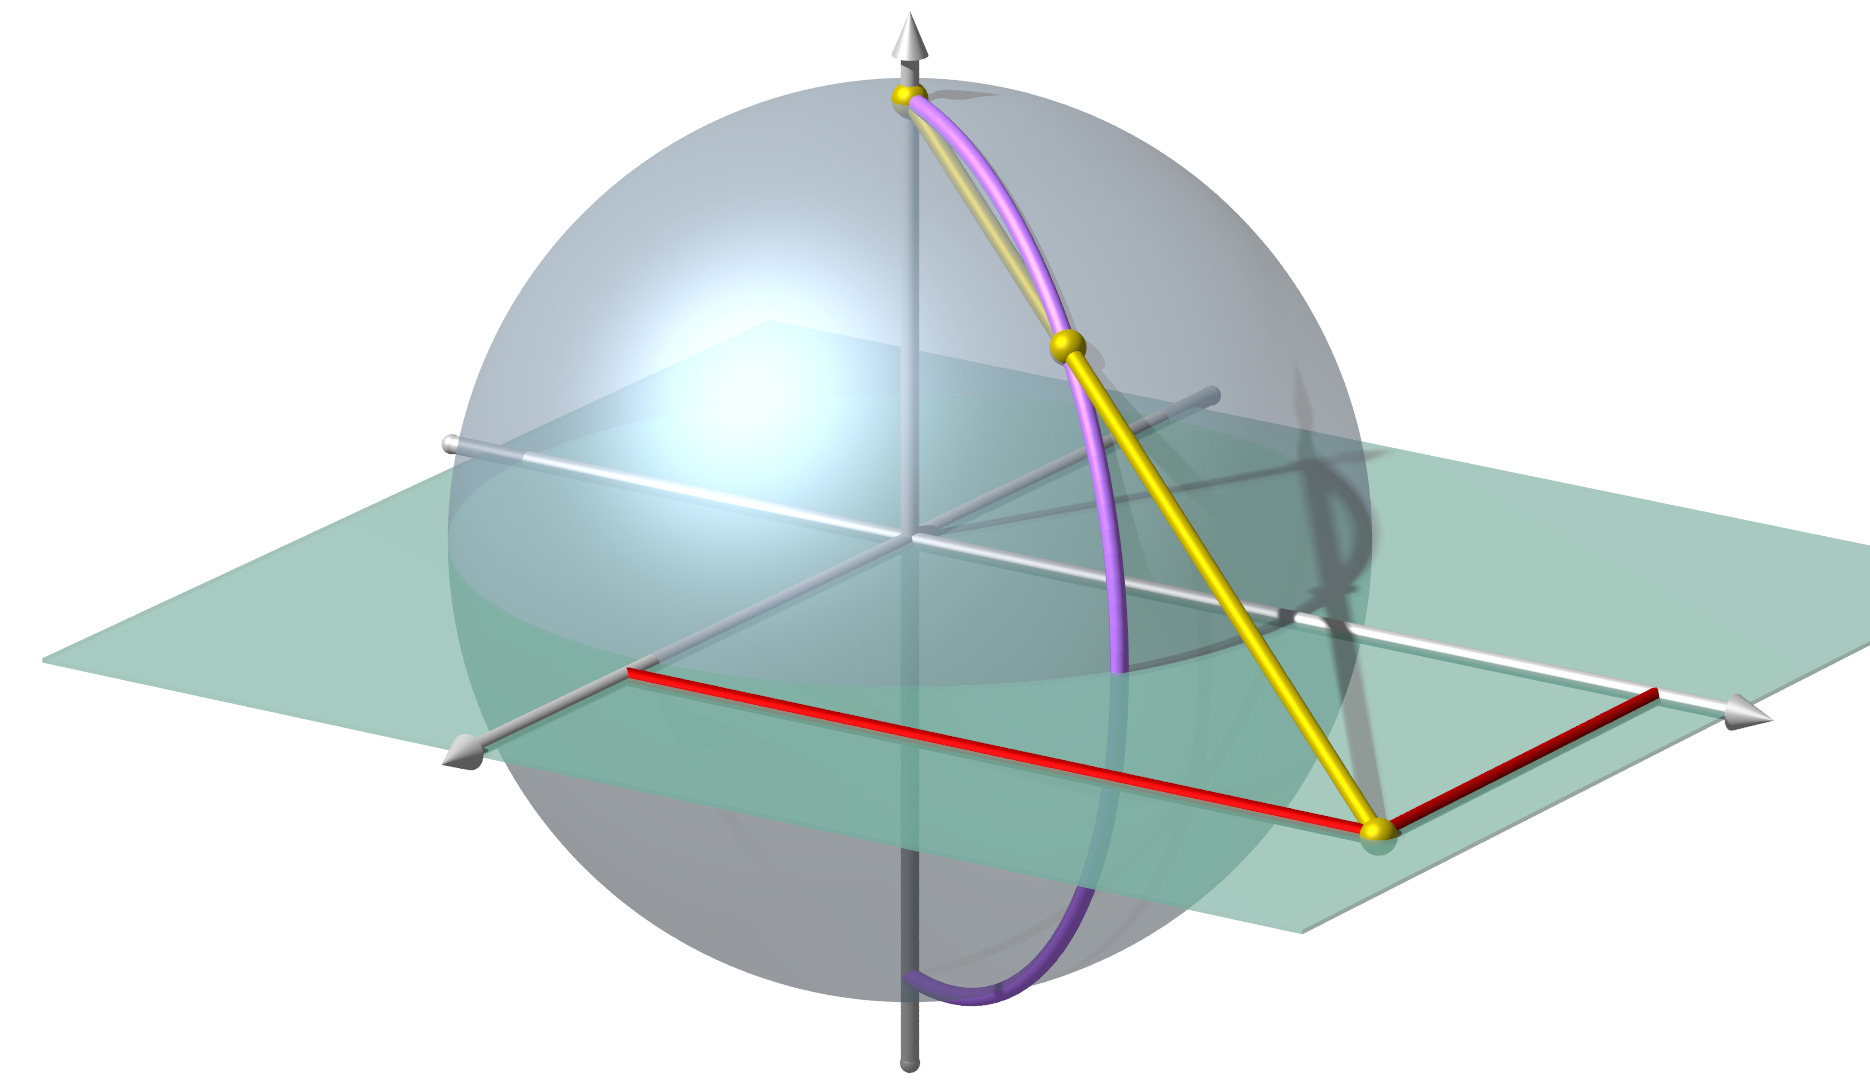
\includegraphics[width=8.3cm]{stereographisch.jpg}};
\node at (0.7,1) {$P=(x,y,z)$};
\node at (1.2,-1.6) {$P'$};
\node at (-1.2,2) {$N$};
\node at (-3.2,-1) {$x^1$};
\node at (3.2,-0.8) {$x^2$};
\node[color=darkred] at (-0.5,-1.3) {$x^2$};
\node[color=darkred] at (2.1,-1.1) {$x^1$};
\end{scope}

\begin{scope}[xshift=-3.3cm]
\begin{scope}
\clip (-0.1,-2.1) rectangle (2,2.1);
\draw[color=gray!40] (0,0) circle[radius=2];
\draw (0,0) ellipse(1 and 2);
\end{scope}
\draw[->] (-0.1,0) -- (4.5,0) coordinate[label={$x^1$}];
\draw[->] (0,-2.2) -- (0,2.3) coordinate[label={right:$z$}];
\fill[color=darkred] (2.2,0) circle[radius=0.08];
\node[color=darkred] at (2.2,0) [above right] {$P'$};
\fill[color=darkred] ({cos(2*\w-90)},{2*sin(2*\w-90)}) circle[radius=0.08];
\node[color=darkred] at ({cos(2*\w-90)},{2*sin(2*\w-90)}) [above right] {$P$};
\draw[color=darkred] (0,2) -- (2.2,0);
\draw[color=darkred,line width=0.3pt]
	(0,{2*sin(2*\w-90)}) -- ({cos(2*\w-90)},{2*sin(2*\w-90)});
\node[color=darkred] at ({0.5*cos(2*\w-90)},{2*sin(2*\w-90)}) [below] {$x$};
\draw[color=darkred] (0,0) -- (2.2,0);
\node[color=darkred] at (1.5,0) [below] {$x^1$};
\node[color=darkred] at (0,{2*sin(2*\w-90)}) [left] {$z$};
\node at (0,2) [left] {$1$};
\end{scope}

\begin{scope}[xshift=3.3cm]
\begin{scope}
\clip (-0.1,-2.1) rectangle (2,2.1);
\draw[color=gray!40] (0,0) circle[radius=2];
\draw (0,0) ellipse(1.732 and 2);
\end{scope}
\draw[->] (-0.1,0) -- (4.5,0) coordinate[label={$x^2$}];
\draw[->] (0,-2.2) -- (0,2.3) coordinate[label={right:$z$}];
\fill[color=darkred] (3.81,0) circle[radius=0.08];
\node[color=darkred] at (3.81,0) [above right] {$P'$};
\draw[color=darkred] (0,2) -- (3.81,0);
\fill[color=darkred]
	({sqrt(3)*cos(2*\w-90)},{2*sin(2*\w-90)}) circle[radius=0.08];
\node[color=darkred] at ({sqrt(3)*cos(2*\w-90)},{2*sin(2*\w-90)})
	[above right] {$P$};
\draw[color=darkred,line width=0.3pt]
	(0,{2*sin(2*\w-90)}) -- ({sqrt(3)*cos(2*\w-90)},{2*sin(2*\w-90)});
\node[color=darkred] at
	({0.5*sqrt(3)*cos(2*\w-90)},{2*sin(2*\w-90)})
	[below] {$y$};
\draw[color=darkred] (0,0) -- (3.81,0);
\node[color=darkred] at (3,0) [below] {$x^2$};
\node[color=darkred] at (0,{2*sin(2*\w-90)}) [left] {$z$};
\node at (0,2) [left] {$1$};
\end{scope}

\end{tikzpicture}
\end{document}

